\documentclass[11pt]{amsart}
%prepared in AMSLaTeX, under LaTeX2e
\addtolength{\oddsidemargin}{-.55in} 
\addtolength{\evensidemargin}{-.55in}
\addtolength{\topmargin}{-.2in}
\addtolength{\textwidth}{1.0in}
\addtolength{\textheight}{.4in}

\renewcommand{\baselinestretch}{1.1}

\usepackage{verbatim,fancyvrb,xspace}

\usepackage{palatino,amssymb}

\usepackage{tikz}
\usetikzlibrary{arrows.meta}

\newtheorem*{thm}{Theorem 16.0}
\newtheorem*{defn}{Definition}
\newtheorem*{example}{Example}
\newtheorem*{problem}{Problem}
\newtheorem*{remark}{Remark}

\usepackage{xspace}

\newcommand{\mfile}[2]{\bigskip
\begin{quote}
\VerbatimInput[frame=single,framesep=3mm,label=\fbox{\normalsize \textsl{\,#2\,}},fontfamily=courier,fontsize=\scriptsize]{#1}
\end{quote}
}

%\usepackage[final]{graphicx}

\usepackage[pdftex, colorlinks=true, plainpages=false, linkcolor=blue, citecolor=red, urlcolor=blue]{hyperref}

% macros
\newcommand{\bc}{\mathbf{c}}
\newcommand{\br}{\mathbf{r}}
\newcommand{\bv}{\mathbf{v}}
\newcommand{\bx}{\mathbf{x}}
\newcommand{\by}{\mathbf{y}}

\newcommand{\CC}{\mathbb{C}}
\newcommand{\RR}{\mathbb{R}}
\newcommand{\ZZ}{\mathbb{Z}}

\newcommand{\eps}{\epsilon}
\newcommand{\grad}{\nabla}
\newcommand{\lam}{\lambda}
\newcommand{\lap}{\triangle}

\newcommand{\ip}[2]{\ensuremath{\left<#1,#2\right>}}

%\renewcommand{\det}{\operatorname{det}}
\newcommand{\onull}{\operatorname{null}}
\newcommand{\rank}{\operatorname{rank}}
\newcommand{\range}{\operatorname{range}}

\newcommand{\prob}[1]{\bigskip\noindent\textbf{#1.}\quad }
\newcommand{\exer}[2]{\prob{Exercise #2 in Lecture #1}}

\newcommand{\pts}[1]{(\emph{#1 pts}) }
\newcommand{\epart}[1]{\medskip\noindent\textbf{(#1)}\quad }
\newcommand{\ppart}[1]{\,\textbf{(#1)}\quad }

\newcommand{\Matlab}{\textsc{Matlab}\xspace}
\newcommand{\Octave}{\textsc{Octave}\xspace}
\newcommand{\Python}{\textsc{Python}\xspace}

\DefineVerbatimEnvironment{mVerb}{Verbatim}{numbersep=2mm,
frame=lines,framerule=0.1mm,framesep=2mm,xleftmargin=4mm,fontsize=\footnotesize}

\newcommand{\ema}{\emach}
\newcommand{\emach}{\eps_{\!_{\text{m}}}}


\begin{document}
\scriptsize \noindent Math 661 Optimization (Bueler) \hfill 1 September, 2016
\normalsize

\medskip\bigskip
\Large
\centerline{A brute-force solution to problem ``\texttt{beam}''}

\bigskip\medskip
\normalsize

\thispagestyle{empty}

As noted in the ``Five example optimization problems'' handout, problem \texttt{beam} is intrinsically infinite-dimensional.

The set of possible inputs to the functional $I[h]$ is
    $$\mathcal{X} = \left\{f \,:\, f'' \text{ is square-integrable on } [0,\pi] \text{ and also } f(0)=f(\pi)=0\right\}.$$
This is a real vector space of functions.\footnote{So that, for example, given any pair of functions $f_1,f_2 \in \mathcal{X}$, and any real numbers $a_1,a_2$, the linear combination $a_1 f_1 + a_2 f_2$ is also in $\mathcal{X}$.}  Why is $\mathcal{X}$ infinite-dimensional, you say?  The answer is that you cannot specify each element using a fixed, finite number of coefficients.\footnote{If it were possible, the number of such coefficients would be the dimension of $\mathcal{X}$.}

For example, and as a hint about the solution method adopted below, the following infinite list of functions live in $\mathcal{X}$:
    $$S = \{\sin x, \sin 2 x, \sin 3 x, \sin 4 x, \dots\} \subset \mathcal{X}.$$
This set is linearly-independent; that is, on cannot write one element of $S$, say $\sin k x$, exactly as a finite linear combination of other elements of the set $S$.  In the appropriate senses, $S$ is a basis for $\mathcal{X}$ and it is an orthogonal set.  For example---this is an instance of Fourier series---the function $f(x) = x (\pi-x)$ is in $\mathcal{X}$ and, on the other hand, there are coefficients $a_k$ so that\footnote{A few points extra credit will be given to anyone who computes the coefficients $a_k$ exactly, and then plots a finite Fourier sum $f_N(x) = \sum_{k=1}^N a_k \sin k x$ showing that the computed coefficients are likely to be correct.}
    $$f(x) = x (\pi-x) = \sum_{k=1}^\infty a_k \sin k x \in \mathcal{X}.$$
But one cannot (exactly) write this $f(x)$ without an infinite sum.

Despite being infinite-dimensional, this kind of beam problem is completely standard in the engineering and physics literature; it is a problem in the \emph{calculus of variations}.  Because of the infinite-dimensionality, only an approximation of the solution can be computed in a finite amount of solution time.\footnote{Actually, this approximate-only status already holds for problem \texttt{calcone}, which is in one-dimension.  In theory the exact solutions of \texttt{fit}, \texttt{salmon}, and \texttt{tsp} are all possible in finite time.  Do you see why for \texttt{fit}?}

The problem is constrained, however, so the solution cannot be just anywhere in the infinite-dimensional vector space $\mathcal{X}$.  The solution lives in an infinite-dimensional convex\footnote{A few points extra credit for proving it is convex.} subset of $\mathcal{X}$:
    $$\mathcal{K} = \left\{f \in \mathcal{X} \,:\, 0.9 \le f(1) \le 1.1 \text{ and } 1.2 \le f(2) \le 1.4 \text{ and } 0.4 \le f(3) \le 0.6\right\}.$$
This is the \emph{feasible set}.  It is like a polyhedron; it is a \emph{polytope} in $\mathcal{X}$.

For now we just want a method that finds an acceptable approximate solution, even if by brute-force.  So we restrict our functions to a five-dimensional (5D)\footnote{It can be $N$ dimensional for any $N$ \dots but the number of (search) grid points goes up exponentially with $N$!  The value $N=5$ represents a trial-and-error-determined compromise between answer quality and execution time.  Strategies in Chapter 16 will overcome this difficulty.} space of truncated Fourier sine series:
    $$\mathcal{X}_5 = \RR^5 = \{[c_1\, c_2\, c_3\, c_4\, c_5]\},$$
where $c\in \mathcal{X}_5$ represents the function $h(x) = \sum_{k=1}^5 c_k \sin k x \in \mathcal{X}$. Using trigonometry we can calculate $I[h]$ for a function $h(x)$ from $\mathcal{X}_5$ \emph{exactly}:
\small
\begin{align*}
I[h] &= \frac{1}{2} \int_0^\pi |h''(x)|^2\,dx = \frac{1}{2} \int_0^\pi \left(- \sum_{k=1}^5 k^2 c_k \sin k x\right)^2\,dx = \frac{1}{2} \sum_{j=1}^5  \sum_{k=1}^5 c_j c_k j^2 k^2 \int_0^\pi \sin j x\sin k x\,dx \\
     &= \frac{1}{4} \sum_{j=1}^5  \sum_{k=1}^5 c_j c_k j^2 k^2 \int_0^\pi \cos((j-k) x) - \cos((j+k) x)\,dx = \frac{1}{4} \sum_{j=1}^5  \sum_{k=1}^5 c_j c_k j^2 k^2 \left(\pi \delta_{jk} - 0\right) = \frac{\pi}{4} \sum_{k=1}^5 k^4 c_k^2.
\end{align*}
\normalsize
(This calculation, which uses the identity $\sin\alpha\sin\beta = \frac{1}{2} \cos(\alpha-\beta) -  \frac{1}{2} \cos(\alpha+\beta)$, will not surprise those who have used Fourier series before.)  The constraint ``$0.9 \le h(1) \le 1.1$'' can be enforced in $\mathcal{X}_5$ by using the formula $h(x) = \sum_{k=1}^5 c_k \sin k x$ and evaluating at $x=1$, and similarly for $x=2,3$.

The approximating 5D optimization problem is now in a form close to (1.1) from the textbook:
    $$\min_{c \in \RR^5} I_5(c) \qquad \text{ subject to } \qquad \begin{matrix}
    0.9 \le \sum_{k=1}^5 c_k \sin k   \le 1.1 \\
    1.2 \le \sum_{k=1}^5 c_k \sin 2 k \le 1.4 \\
    0.4 \le \sum_{k=1}^5 c_k \sin 3 k \le 0.6
    \end{matrix}$$
where
    $$I_5(c) = \frac{\pi}{4} \sum_{k=1}^5 k^4 c_k^2.$$
This is called a \emph{quadratic programming problem}; see Chapter 16 of the textbook.  Let $\mathcal{K}_5 \subset \RR^5$ be the (convex) set where the constraints are satisfied; this is the \emph{feasible} set for the approximate optimization problem.  Our problem is now a constrained, 5D version of the unconstrained 3D problem \texttt{fit}.

We do not know, however, which of the inequality constraints is active (i.e.~the inequality is equality) when $c$ is the solution of the problem.  Taking partial derivatives of $I_5$ and setting them to zero just yields $c=0$, which does not satisfy the constraints, so $c=0$ is not the solution.  We do not know the shape, in five dimensions, of the subset of $\RR^5$ which satisfies the constraints; it is a 5D polytope.  Thus we will solve the five-dimensional problem by brute force, searching on a grid of points inside a box in $\RR^5$, in the hope that we cover enough of the constrained set to get near the minimum.  Only trial-and-error can make this possible.

The proposed box, based on trial-and-error, is
	$$\mathcal{B}_5 = \left\{0 \le c_1 \le 2, \,
	                         -1 \le c_2 \le 1, \,
	                         -0.5 \le c_3 \le 0.5, \,
	                         -0.2 \le c_4 \le 0.2, \,
	                         -0.2 \le c_5 \le 0.2\right\}.$$

The code below puts a grid with a given spacing on this box and then evaluates $I_5(c)$ at every point on the grid.  I have also posted a code \texttt{plotbeam.m} which plots the tent pole corresponding to a given $c\in \RR^5$.  Running the code with a grid of sufficient coarseness to give a reasonable execution time, namely a few minutes, looks like

\medskip
\begin{Verbatim}[fontfamily=courier,fontsize=\scriptsize]
>> [z h] = beam(0.05)
...
z =  5.8316
h =
  1.40000  -0.30000  0.15000  -0.05000  0.05000
>> plotbeam(h)
\end{Verbatim}

\medskip
\noindent Thus $c_1=1.4$, $c_2=-0.3$, $c_3=0.15$, $c_4=-0.05$, and $c_5=0.05$ from this brute-force search, giving minimum value $I_5(c)=5.8316$.  (During the run the code shows characters \texttt{.}/\texttt{o}/\texttt{*} for progress made so far, including the best solution so far; this is not shown.)  The last ``\texttt{plotbeam}'' command plots the figure at the end, which I believe is pretty close to the solution!

\bigskip

\mfile{matlab/beam.m}{beam.m}

\bigskip
\begin{center}
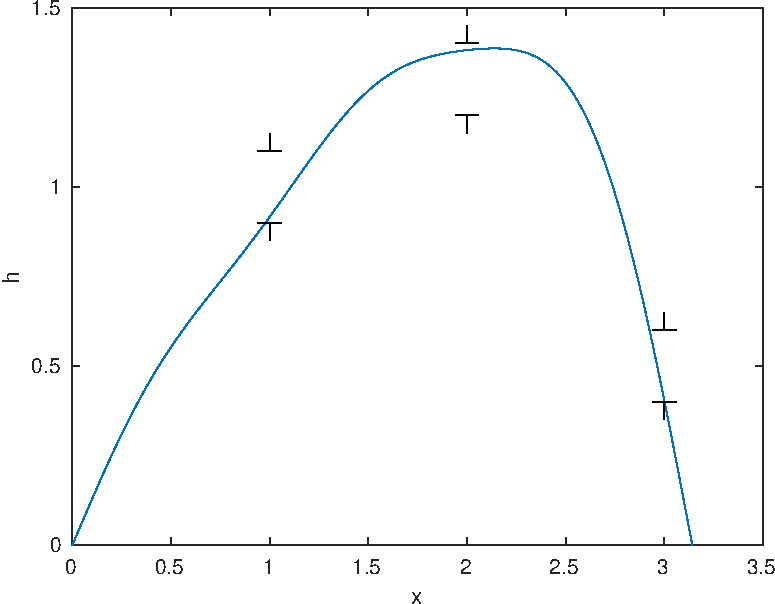
\includegraphics[width=0.65\textwidth]{beam-soln-gates}
\end{center}

\end{document}

